% !TEX program = xelatex
\documentclass{ctexart}
\usepackage{xcolor} % 在latex中使用颜色
\usepackage{booktabs,tabularx,multicol} % 制作表格
\usepackage{framed} % 制作文本框
\usepackage{amsmath,amsthm,amssymb,amsfonts}    % 数学符号与字体
\usepackage{hyperref}   % 添加超链接
\usepackage[left=2.0cm, right=2.0cm, top=2.5cm, bottom=2.5cm]{geometry} % 调整页边距
\usepackage{appendix}   % 附录环境
\usepackage{subfig,graphicx}    % 插入照片

%---------------优雅的插入MATLAB代码---------%
\usepackage{listings,matlab-prettifier} % MATLAB 美化包
\lstset{
        style=Matlab-editor,
        basicstyle=\mlttfamily,
        escapechar=`,
        numbers      = left,
        numbersep    = 5pt,
        numberstyle  = \small\color{red},
        frame        = single,
        keepspaces   = true,
        tabsize      = 4,
        breaklines = true,
}
%-------------标题-------------%
\author{201931071225\quad 201931071332}
\date{\today}
\title{利用直接差分法分析微分方程边值问题}

%-----------做一些设置-----------%
\numberwithin{equation}{section}    % 公式标号与section的编号挂钩
\punctstyle{kaiming}    % 调整标点符号大小

%------------自定义一些命令------------%
\newcommand{\upcite}[1]{\textsuperscript{\textsuperscript{\cite{#1}}}}
\newcommand*{\dif}{\mathop{}\!\mathrm{d}}
\def\degree{${}^{\circ}$}

%---------配置环境------------%
\definecolor{shadecolor}{RGB}{241,241,255}
\newcounter{problemname}
\newenvironment{problem}{\begin{shaded}\stepcounter{problemname}\par\noindent\textbf{题目\arabic{problemname}. }}{\end{shaded}\par}
\newenvironment{solution}{\par\noindent\textbf{解答. }}{\par}
\newenvironment{note}{\par\noindent\textbf{题目\arabic{problemname}的注记. }}{\par}

%-------------可控列宽的表格--------%
\newcolumntype{R}[1]{>{\raggedright\arraybackslash}p{#1}}
\newcolumntype{C}[1]{>{\centering\arraybackslash}p{#1}}
\newcolumntype{L}[1]{>{\raggedleft\arraybackslash}p{#1}}



\begin{document}

\maketitle
\tableofcontents
\newpage
\section{题目}
\begin{equation}
    \left\{\begin{aligned}
            L u&=-\frac{\dif}{\dif x}\left(x \frac{\dif u}{\dif x}\right)+\frac{\dif u}{\dif x}+u=x \cos x+\cos x, x \in[0, \pi] \\
            u(0)&=1; u(\pi)=-1
    \end{aligned}\right.
\end{equation}
简单推导可以得到
\begin{equation}
    u- x\frac{\dif^2u}{\dif x^2}= x\cos x+\cos x
\end{equation}
\section{离散形式}
利用直接差分法可以得到:
\begin{equation}
    \begin{aligned}
    &u_i - x_i\frac{u_{i+1}-2u_i+u_{i-1}}{h^2}=x_i\cos x_i+\cos x_i,\quad i = 1,2,\cdots,n-1\\
    &u_0 = 1,u_n=-1,h = \frac{\pi}{n}
    \end{aligned}
\end{equation}
再整理得到
\begin{equation}
    \begin{aligned}
    &-\frac{x_i}{h^2}u_{i+1}+(1+\frac{2x_i}{h^2})u_i-\frac{x_i}{h^2}u_{i-1}=x_i\cos x_i+\cos x_i,\quad i = 1,2,\cdots,n-1\\
    &u_0 = 1,u_n=-1,h = \frac{\pi}{n}
    \end{aligned}
\end{equation}
写成矩阵形式为

\begin{equation}
    \begin{bmatrix}
        1&0&0&\cdots&0&0&0\\
        -\frac{x_1}{h^2}&(1+\frac{2x_1}{h^2})&-\frac{x_1}{h^2}&\cdots&0&0&0\\
        0&-\frac{x_2}{h^2}&(1+\frac{2x_2}{h^2})&\cdots&0&0&0\\
        \vdots  & \vdots  & \vdots & &\vdots &\vdots & \vdots\\
        0&0&0&\cdots&(1+\frac{2x_{n-2}}{h^2})&-\frac{x_{n-1}}{h^2}&0\\
        0&0&0&\cdots&-\frac{x_{n-1}}{h^2}&(1+\frac{2x_{n-1}}{h^2})&-\frac{x_{n-1}}{h^2}\\
        0&0&0&\cdots&0&0&1\\
    \end{bmatrix}
    \begin{bmatrix}
        u_0\\
        u_1\\
        u_2\\
        \vdots\\
        u_{n-2}\\
        u_{n-1}\\
        u_n
    \end{bmatrix}
    =
    \begin{bmatrix}
        (x_0+1)\cos x_0\\
        (x_1+1)\cos x_1\\
        (x_2+1)\cos x_2\\
        \vdots\\
        (x_{n-2}+1)\cos x_{n-2}\\
        (x_{n-1}+1)\cos x_{n-1}\\
        (x_n+1)\cos x_n\\
    \end{bmatrix}
\end{equation}
\section{代码}
\lstinputlisting[caption={\bf main.m},]{code/main.m}
\begin{figure}[htp]
    \centering
    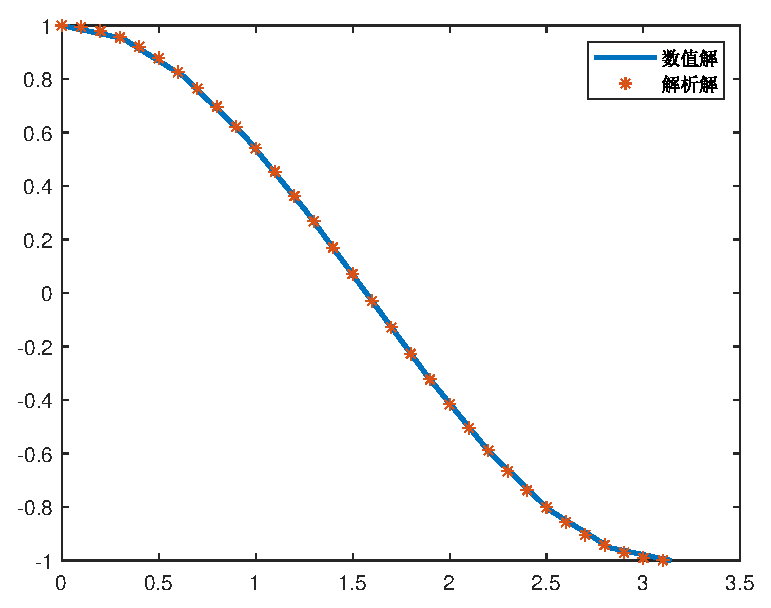
\includegraphics[width=0.7\linewidth]{fig/pic.eps}
\end{figure}

\section{误差分析}

有限差分法的潜在的误差来源是中心差分公式的截断误差,以及在求解方程组时带来的误差。此处我们调用的是 MATLAB 内置的求解方程组的算法,精度较高。因此,截断误差占优,误差是 $O(h^2)$,因而我们期望随着子区间 $n + 1$ 升高,误差降低为 $O(h^2)$.

我们对于此问题测试了这种方差,图显示了最大误差对于不同 n 取值对应的解的误差 E 的取值。在log-log 图中,$\lg(E)-\lg(n)$ 是一条斜率为 -2 的直线,意味着,$\lg E \thickapprox  α + b \lg n$, 其中 b = −2;换句话说,与我们预期一致,误差为 $E \thickapprox Kn^{−2}$
\begin{figure}[htp]
    \centering
    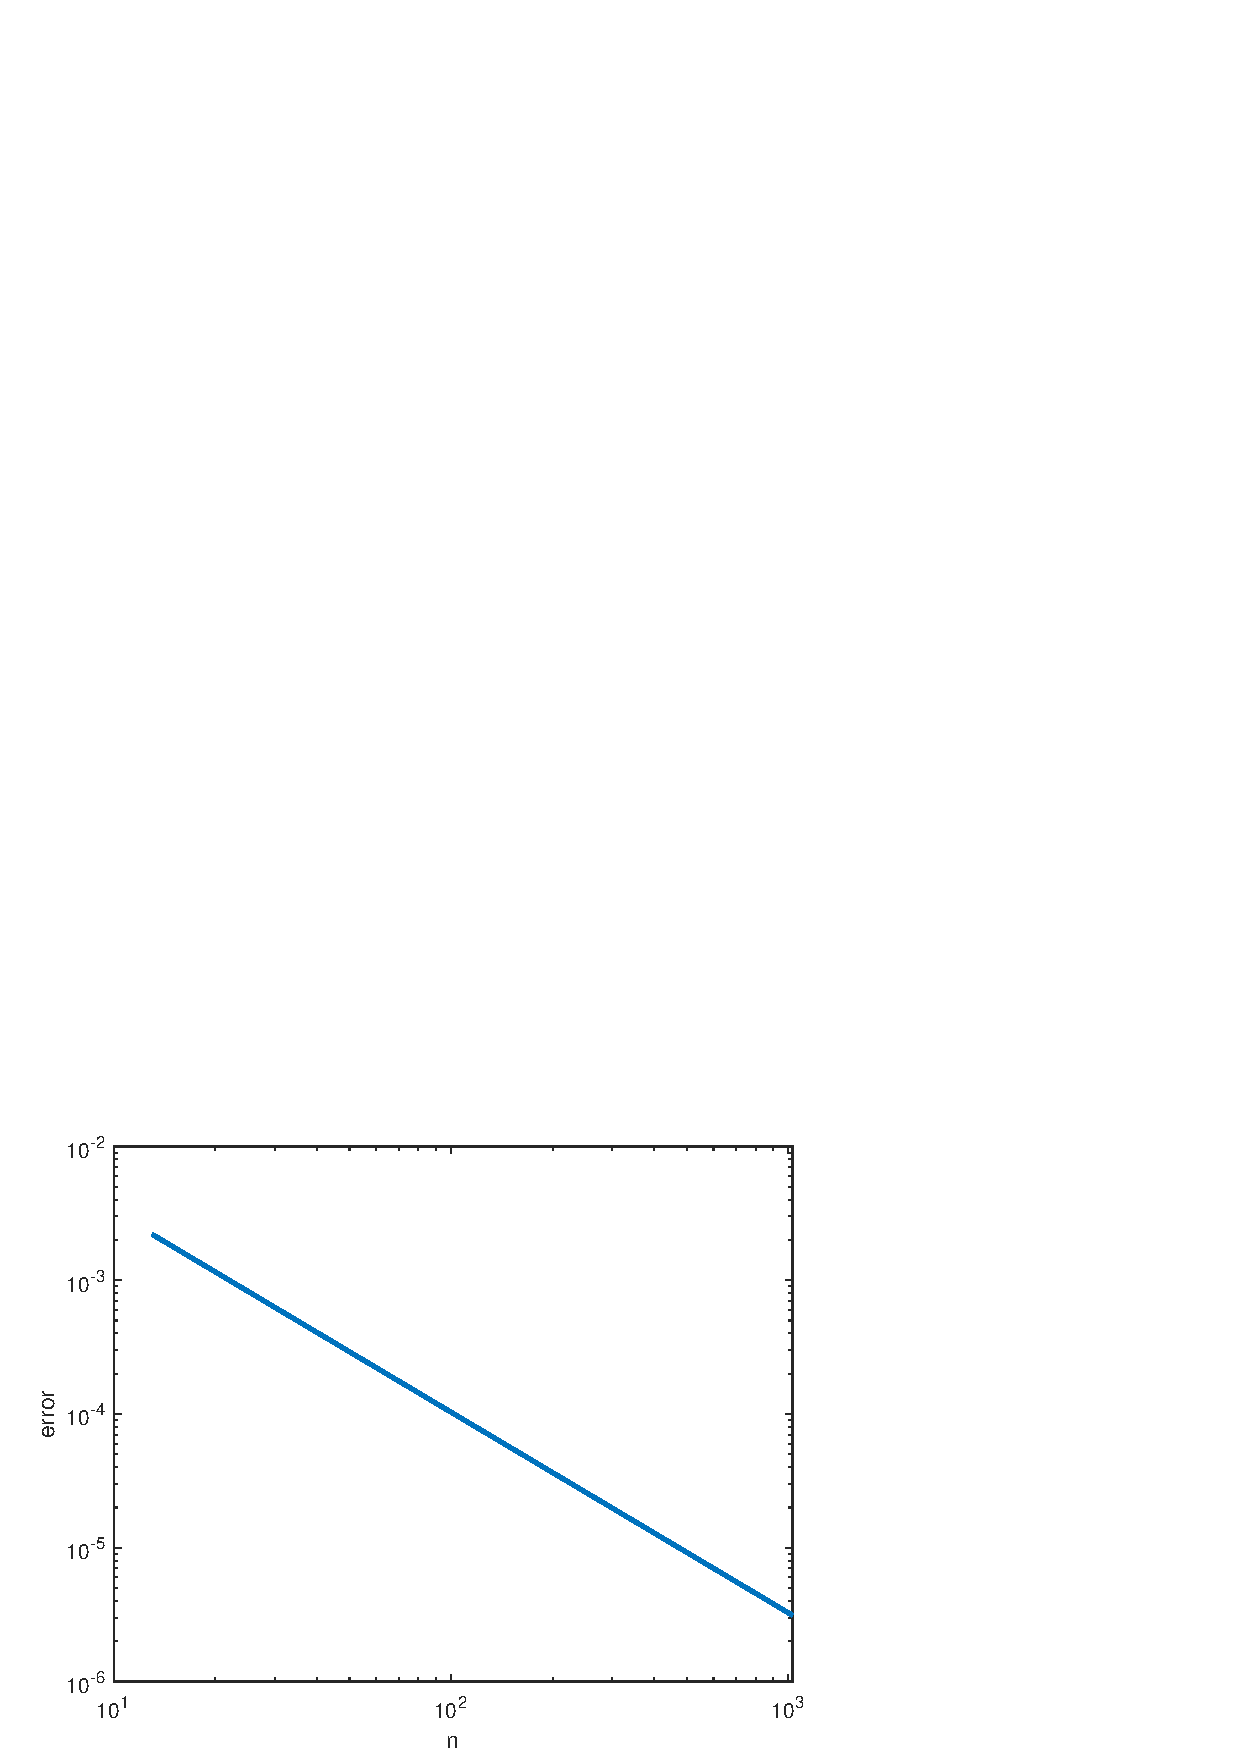
\includegraphics[width=0.7\linewidth]{fig/pic2}
\end{figure}

\end{document}